\section*{Appendix}
\appendix
\section{Implementation Details}
\subsection{Model Architecture Details} 

In the first learning stage, we aim to predict the task class label given the observations $\left\{V_s, V_g\right\}$. We employ a simple 4-layer transformer model for this task and use cross-entropy loss to train the model by comparing its output with the ground truth task class labels.

The classifier is a neural network based on the transformer architecture. It first embeds the input data through a linear layer, after which the embedded data is processed by multiple stacked transformer encoder layers. The output of the encoder layers is averaged and then passed through a series of fully connected layers with ReLU activation functions. Finally, the processed data is passed through a linear layer to generate the final output. Dropout layers are applied throughout the model to prevent overfitting. 

Next, our main model is based on a 3-layer U-Net~\citep{ronneberger2015u}, similar to \citet{wang2023pdpp}, but adapted for temporal action prediction. Each layer consists of two residual temporal blocks~\citep{he2016deep}, followed by either downsampling or upsampling. Each residual temporal block includes two convolutional layers, group normalization~\citep{wu2018group}, Mish activation~\citep{misra2019mish}, and a cross-attention module for feature fusion. Temporal embeddings are generated via a fully connected layer and added to the output of the first convolution. To handle the short planning horizon ($T = \{3, 4, 5, 6\}$), we employ 1D convolutions with a kernel size of 2, stride of 1, and no padding for downsampling/upsampling used by \citet{wang2023pdpp}, instead of the max-pooling approach, ensuring the horizon length remains unchanged. The middle block consists of only two residual temporal blocks.

The input matrix $\hat{x}_n$ is a concatenation of the task class, action sequences, and observation features, with a dimension of $fusion\_dim = C + A + O$, where $C$, $A$, and $O$ represent the number of task classes, action labels, and visual features, respectively. During the downsampling phase, the input is embedded through $[fusion\_dim \to 256 \to 512 \to 1024]$, with the reverse process occurring during the upsampling phase.

The latent space temporal logical interpolation module consists of three main components: an observation encoder, a latent space interpolator, and transformer encoder blocks. The observation encoder reduces the input dimensionality using two 1D convolutional layers with ReLU activations. The latent space interpolator generates intermediate features between two encoded representations via linear interpolation, guided by a learnable linear layer initialized with matrix $\tau$. The generated matrix is passed through a Sigmoid function to compute $I_j$. Finally, standard transformer encoder blocks apply attention mechanisms to enhance the temporal logical relationships in $F_j$, ultimately producing transformed latent features with a shape of $[M, O]$, where $M$ refers to the number of residual temporal blocks in the U-Net.


For the diffusion process, we employ a cosine noise schedule to generate $\{\beta_n\}_{n=1}^N$, which controls the amount of noise added at each step. These values correspond to the variance of the Gaussian noise introduced at each stage of diffusion.


\subsection{Dataset Details} 
Each video in the dataset is annotated with action labels and their corresponding temporal boundaries, denoted as $\{s_i, e_i\}$ for the $i$-th action, where $s_i$ and $e_i$ represent the start and end times, respectively. The total number of actions in the dataset is denoted as $Num$. We extract step sequences $a_{t:(t+T-1)}$ from the videos, with the horizon $T$ ranging from 3 to 6. Following the method in previous work~\citep{wang2023pdpp}, action sequences $\{[a_t, \ldots, a_{t+T-1}]\}_{t=1}^{Num-T+1}$ are generated by sliding a window of size $T$ over the $Num$ actions. For each sequence, the video clip feature at the start time of action $a_t$ is used as the starting observation $V_s$, and the clip feature at the end time of action $a_{t+T-1}$ is used as the goal state $V_g$. Both clips are 3 seconds in duration. The start and end times of each sequence are rounded to $\lfloor s_t \rfloor$ and $\lceil e_{t+T-1} \rceil$, respectively, with the clip features between these times used as $V_s$ and $V_g$.

For the CrossTask dataset, we consider two types of pre-extracted features: (1) the 3200-dimensional features provided by the dataset, which combine I3D, ResNet-152, and audio VGG features~\citep{carreira2017quo,he2016deep,hershey2017cnn}, and (2) features extracted using an encoder trained on the HowTo100M dataset~\citep{miech2019howto100m}, as used in~\citep{wang2023pdpp}. We utilize the latter due to its smaller size. For the COIN and NIV datasets, we also use HowTo100M features~\citep{wang2023pdpp} to maintain consistency and ensure fair comparison.



\subsection{Details of Metrics }
Previous works~\citep{chang2020procedure, bi2021procedure, sun2022plate} computed the mIoU metric over mini-batches, averaging the results across the batch size. However, this method introduces variability depending on the batch size. For instance, if the batch size equals the entire dataset, all predicted actions may be considered correct. In contrast, using a batch size of one penalizes any mismatch between predicted and ground-truth sequences. To address this issue, we follow \citet{wang2023pdpp} by standardizing mIoU calculation, computing it for each individual sequence and then averaging the results, effectively treating the batch size as one. However, this approach may result in our mIoU scores being lower than those reported by others.


\subsection{Training Details} 
Following \citet{wang2023pdpp}, we employ a linear warm-up strategy to train our model, with specific protocols adjusted for different datasets. For the CrossTask dataset, we set the diffusion steps to 250 and train for 20,000 steps. The learning rate is linearly increased to \(5 \times 10^{-4}\) over the first 3,333 steps, then halved at steps 8,333, 13,333, and 18,333. For the NIV dataset, with 50 diffusion steps, training lasts for 5,000 steps. The learning rate ramps up to \(3 \times 10^{-4}\) over the first 1,000 steps and is reduced by 50\% at steps 2,666 and 4,332. In the larger COIN dataset, we use 300 diffusion steps and train for 30,000 steps. The learning rate increases to \(1 \times 10^{-5}\) in the first 5,000 steps and is halved at steps 12,500, 20,000, and 27,500, stabilizing at \(2.5 \times 10^{-6}\) for the remaining steps. Training is performed using ADAM~\citep{kingma2014adam} on 8 NVIDIA RTX 3090 GPUs.


\subsection{Details of Uncertainty Modeling}
In the main paper, we investigate the probabilistic modeling capability of our model on the CrossTask and COIN datasets, demonstrating that our diffusion-based model can generate both diverse and accurate plans. Here, we provide additional details, results, and visualizations to further illustrate how our model handles uncertainty in procedure planning. 

\textbf{Details of Evaluating Uncertainty Modeling.} For the $Deterministic$ baseline, we sample once to obtain the plan, as the result is fixed when the observations and task class conditions are given. For the $Noise$ baseline and our diffusion-based model, we sample 1,500 action sequences to calculate the uncertainty metrics. To efficiently perform this process, we apply the DDIM~\citep{song2020denoising} sampling method to our model, enabling each sampling process to be completed in 10 steps. This accelerates sampling by 20 times for CrossTask and COIN, and by 5 times for NIV. It is important to note that multiple sampling is only required when evaluating probabilistic modeling—our model can generate a good plan with just a single sample.

\begin{wraptable}{r}{0.45\textwidth}
\vspace{-5mm}
\centering
\caption{The results of uncertain modeling on the COIN dataset.}
\label{tab:unc-COIN}
\scalebox{0.87}{
\begin{tabular}{l l c c}
\toprule
Metric & Method & $T=3$ & $T=4$  \\ 
\midrule
\multirow{3}*{KL-Div $\downarrow$}
&  Deterministic & \textbf{4.47} & \textbf{4.40}\\ 
&  Noise & 5.12 & 4.88\\ 
&  Ours & \underline{4.74} & \underline{4.47} \\ 
\midrule
\multirow{3}*{NLL $\downarrow$}
&  Deterministic & \textbf{5.42} & \textbf{5.81}\\ 
&  Noise & 6.07 & 6.28\\ 
&  Ours & \underline{5.69} & \underline{5.87} \\ 
\midrule
\multirow{3}*{ModePrec $\uparrow$}
&  Deterministic & \textbf{34.04} & \textbf{32.47}\\ 
&  Noise & 23.16 & 22.18 \\ 
&  Ours & \underline{28.83} & \underline{26.91}\\
\midrule
\multirow{3}*{ModeRec $\uparrow$}
&  Deterministic & \textbf{27.41} & \textbf{20.88}\\ 
&  Noise & 21.06 & 15.24 \\ 
&  Ours & \underline{23.27} & \underline{18.14} \\
\bottomrule
\end{tabular}
}
\vspace{-7mm}
\end{wraptable}
\textbf{Additional Results on COIN.} Results on the COIN dataset are presented in \Cref{tab:unc-COIN}. On the COIN dataset, our model underperforms relative to the $Deterministic$ baseline. We attribute this to the shorter action sequences, where reduced uncertainty is more advantageous but less critical for long-horizon procedural planning.

\textbf{Visualizations for Uncertainty Modeling.} In \Cref{fig:visual-3,fig:visual-4,fig:visual-5,fig:visual-6}, we present visualizations of various plans with the same start and goal observations, generated by our masked temporal interpolation diffusion model on CrossTask for different prediction horizons. We have observed that some results contain repeated actions, which is due to the probabilistic nature of our model's prediction method, making repeated action predictions unavoidable. The top five predicted logits for the actions are passed through a softmax function, and the action with the highest probability is selected to form the prediction figures. 

\section{Baseline Methods}
In this section, we describe the baseline methods used in our study.
\begin{itemize}
    \item \textbf{Random Selection.} This method randomly selects actions from the available action space within the dataset to generate plans.
    \item \textbf{Retrieval-Based Approach.} Given the observations \(\{V_s, V_g\}\), this method retrieves the nearest neighbor by minimizing the visual feature distance within the training dataset. The action sequence associated with the retrieved neighbor is then used as the plan.
    \item \textbf{WLT DO \citep{ehsani2018let}.} This method employs a recurrent neural network (RNN) to predict action steps based on the provided observation pairs.
    \item \textbf{UAAA \citep{abu2019uncertainty}.} UAAA is a two-stage approach that uses an RNN-HMM model to predict action steps in an auto-regressive manner.
    \item \textbf{UPN \citep{srinivas2018universal}.} UPN is a path planning algorithm for physical environments that learns a plannable representation to generate predictions. To produce discrete action steps, a softmax layer is appended to the model's output, as described in \citep{chang2020procedure}.
    \item \textbf{DDN \citep{chang2020procedure}.} DDN is an auto-regressive framework with two branches designed to learn an abstract representation of action steps and predict transitions in the feature space.
    \item \textbf{PlaTe \citep{sun2022plate}.} PlaTe extends DDN by incorporating transformer modules into its two branches for prediction tasks. PlaTe uses a different evaluation protocol compared to other models.
    \item \textbf{Ext-GAIL \citep{bi2021procedure}.} Ext-GAIL addresses procedure planning using reinforcement learning. Unlike our approach, Ext-GAIL divides the planning problem into two stages: the first provides long-horizon information, which is then used by the second stage. In contrast, our approach derives sampling conditions directly.
    \item \textbf{P$^3$IV \citep{zhao2022p3iv}.} P$^3$IV is a transformer-based, single-branch model that incorporates a learnable memory bank and an additional generative adversarial framework. Similar to our model, P$^3$IV predicts all action steps simultaneously during inference.
    \item \textbf{PDPP \citep{wang2023pdpp}.} PDPP is a two-branch framework that models temporal dependencies and action transitions using a diffusion process. Like our model, PDPP predicts all actions simultaneously, refining predictions over multiple stages to enhance logical consistency during inference.
    \item \textbf{KEPP \citep{nagasinghe2024not}.} KEPP is a knowledge-enhanced procedure planning system that leverages a probabilistic procedural knowledge graph (P2KG) learned from training plans. This graph acts as a ``textbook'' to guide step sequencing in instructional videos. KEPP predicts all action steps simultaneously with minimal supervision, achieving leading performance.
    \item \textbf{SCHEMA \citep{niu2024schema}.} SCHEMA focuses on procedure planning by learning state transitions. It employs a transformer-based architecture with cross-modal contrastive learning to align visual inputs with text-based state descriptions. By tracking intermediate states, SCHEMA predicts future actions using a large language model to capture temporal dependencies and logical transitions, improving action planning in instructional videos.
\end{itemize}


\section{Additional Ablation Studies}


\textbf{Model Size.} Due to the large size of the COIN dataset, we adjust the model size by modifying the U-Net architecture. As shown in \Cref{tab:dm_combined}, increasing the model size results in higher scores for the COIN dataset. We believe that optimizing the model to be more memory-efficient could further improve performance, which we plan to explore in future work. In \Cref{tab:dm_combined}, increasing the size to 512 does not improve the scores on CrossTask. We believe this suggests overfitting, indicating that a model size of 256 is sufficient for this task.

\begin{table}[htbp]
\centering
\caption{Ablation study on the role of model size on COIN and CrossTask datasets.}
\vspace{2mm}
\scalebox{0.92}{
\begin{tabular}{llccccccc}
\toprule
& & \multicolumn{3}{c}{$T$ = 3} & & \multicolumn{3}{c}{$T$ = 4} \\ 
\cline{3-5} \cline{7-9}
Dataset & Size & SR$\uparrow$ & mAcc$\uparrow$ & mIoU$\uparrow$ & & SR$\uparrow$ & mAcc$\uparrow$ & mIoU$\uparrow$ \\ 
\midrule
\multirow{3}{*}{COIN} 
& 128 & 23.01 & 45.44 & 51.93 & & 19.69 & 45.32 & 55.06 \\
& 256 & \underline{28.84} & \underline{50.44} & \underline{57.86} & & \underline{21.64} & \underline{48.06} & \underline{59.52} \\
& 512 & \textbf{30.90} & \textbf{52.17} & \textbf{59.58} & & \textbf{23.10} & \textbf{49.71} & \textbf{60.78} \\
\midrule
\multirow{3}{*}{CrossTask} 
& 128 & 23.01 & 45.44 & 51.93 & & 19.69 & 45.32 & 55.06 \\
& 256 & \textbf{40.45} & \textbf{67.19} & \textbf{69.17} & & \textbf{24.76} & \textbf{60.69} & \textbf{67.67} \\
& 512 & \underline{37.94} & \underline{65.16} & \underline{67.43} & & \underline{21.97} & \underline{58.30} & \underline{66.15} \\
\bottomrule
\end{tabular}
}
\label{tab:dm_combined}
\end{table}

\begin{table}[htbp]
\centering
\caption{Ablation study on the observation encoder components ($T=3$, CrossTask).}
\vspace{2mm}
\scalebox{0.92}{
\begin{tabular}{lccc}
\toprule
Models & SR$\uparrow$ & mAcc$\uparrow$ & mIoU$\uparrow$ \\ 
\midrule
1 1d conv. layer w/ ReLU & \underline{39.71} & \underline{66.91} & \underline{69.05} \\
2 1d conv. layers w/ ReLU (Ours) & \textbf{40.45} & \textbf{67.19} & \textbf{69.17} \\
3 1d conv. layers w/ ReLU & 36.04 & 64.41 & 66.55 \\
1 1d conv. layer w/o ReLU & 39.32 & 66.70 & 68.91 \\
2 1d conv. layers w/o ReLU & 39.38 & 66.73 & 68.65 \\
3 1d conv. layers w/o ReLU & 37.77 & 65.06 & 67.61 \\
\bottomrule
\end{tabular}
}
\label{tab:encoder_layer}
\end{table}


\textbf{Components of Observation Encoder.} \Cref{tab:encoder_layer} presents the impact of different encoder components. Based on this ablation study, the optimal model consists of two 1D convolution layers with ReLU activation, which achieves the best balance between depth and activation, resulting in the highest scores across all metrics. Adding more layers does not consistently improve performance, and activation functions like ReLU play a key role in enhancing model effectiveness. We believe that ReLU introduces non-linearity, enabling the network to capture temporal latent features more effectively. Moreover, by setting negative values to zero, ReLU promotes sparse activation, which may aid in the extraction and construction of latent features.

\textbf{Transformer Classifier Type.} We conduct ablation studies on the CrossTask and COIN datasets to evaluate the impact of our transformer-based classifier. As shown in \Cref{tab:classifier_crosstask,tab:classifier_coin}, the inclusion of the transformer-based classifier significantly boosts the performance of PDPP. Although the improvements are modest for longer horizons, this highlights the effectiveness of our temporal interpolation module on CrossTask compared to PDPP with the same transformer classifier. However, the classifier's performance may also limit further improvements. Additionally, we observe that even with incorrect task class labels during supervision, the model still achieves strong scores, demonstrating its robustness, fault tolerance, and error correction capabilities. 


\begin{table}[t]
\centering
\caption{Ablation study on the role of classifier type on CrossTask dataset.}
\vspace{-3mm}
\scalebox{0.92}{
\begin{tabular}{lccccccccc}
\toprule
& \multicolumn{3}{c}{$T$ = 3} & & \multicolumn{3}{c}{$T$ = 4} & $T$=5 & $T$ = 6 \\ 
\cline{2-4} \cline{6-8}
{Models}          & SR$\uparrow$ & mAcc$\uparrow$   & mIoU$\uparrow$  &   & SR$\uparrow$    & mAcc$\uparrow$   & mIoU$\uparrow$  & SR$\uparrow$ & SR$\uparrow$ \\ \midrule
{PDPP (Res-MLP)}  & 37.2         & 55.35            & 66.57           &   & 21.48 &  57.82 &  65.13 &  13.58 &  8.47 \\
{PDPP (Transformer)}             & \underline{39.08} & \underline{66.32} & \underline{68.47}  &  &  \underline{22.48} &  \bf 60.72 &  \underline{66.13} &  \underline{13.77} &  \underline{8.63} \\
{MTID (Transformer)}    &   \bf 40.45 & \bf 67.19 & \bf 69.17  &  & \bf 24.76 & \underline{60.69} &  \bf 67.67 & \bf 15.26 & \bf 10.30 \\
\bottomrule
\end{tabular}
}
\label{tab:classifier_crosstask}
\end{table}

\begin{figure}[htbp]
    \centering
    \subfloat[Ablation studies on different complex initialization methods with max value 6.]
    {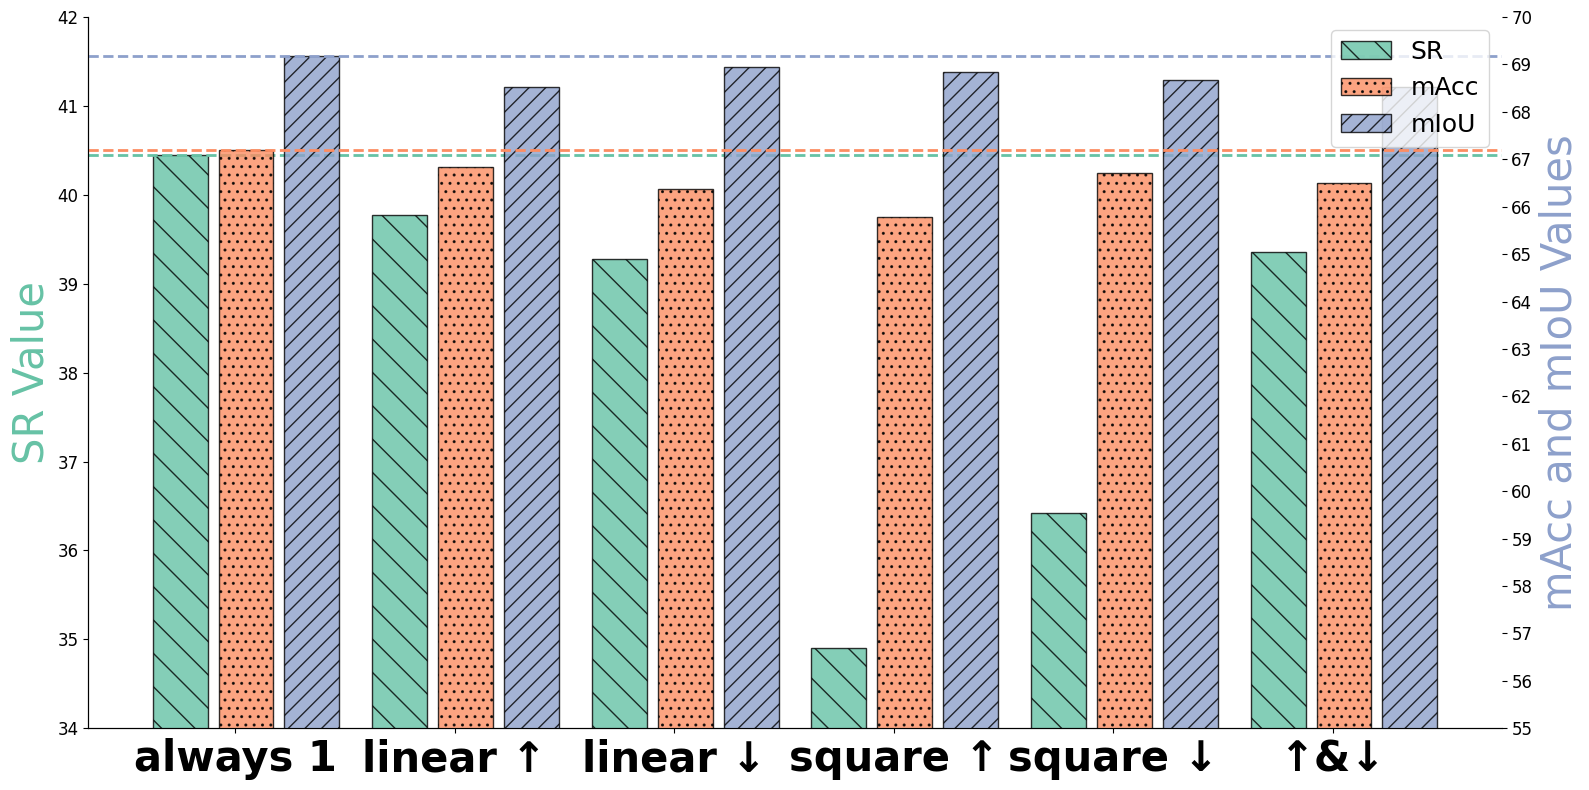
\includegraphics[width=0.45\textwidth]{figures/intx1.png}\label{fig:inxx1}}
    \hfill
    \subfloat[Ablation studies on different complex initialization methods with max value 1.]
    {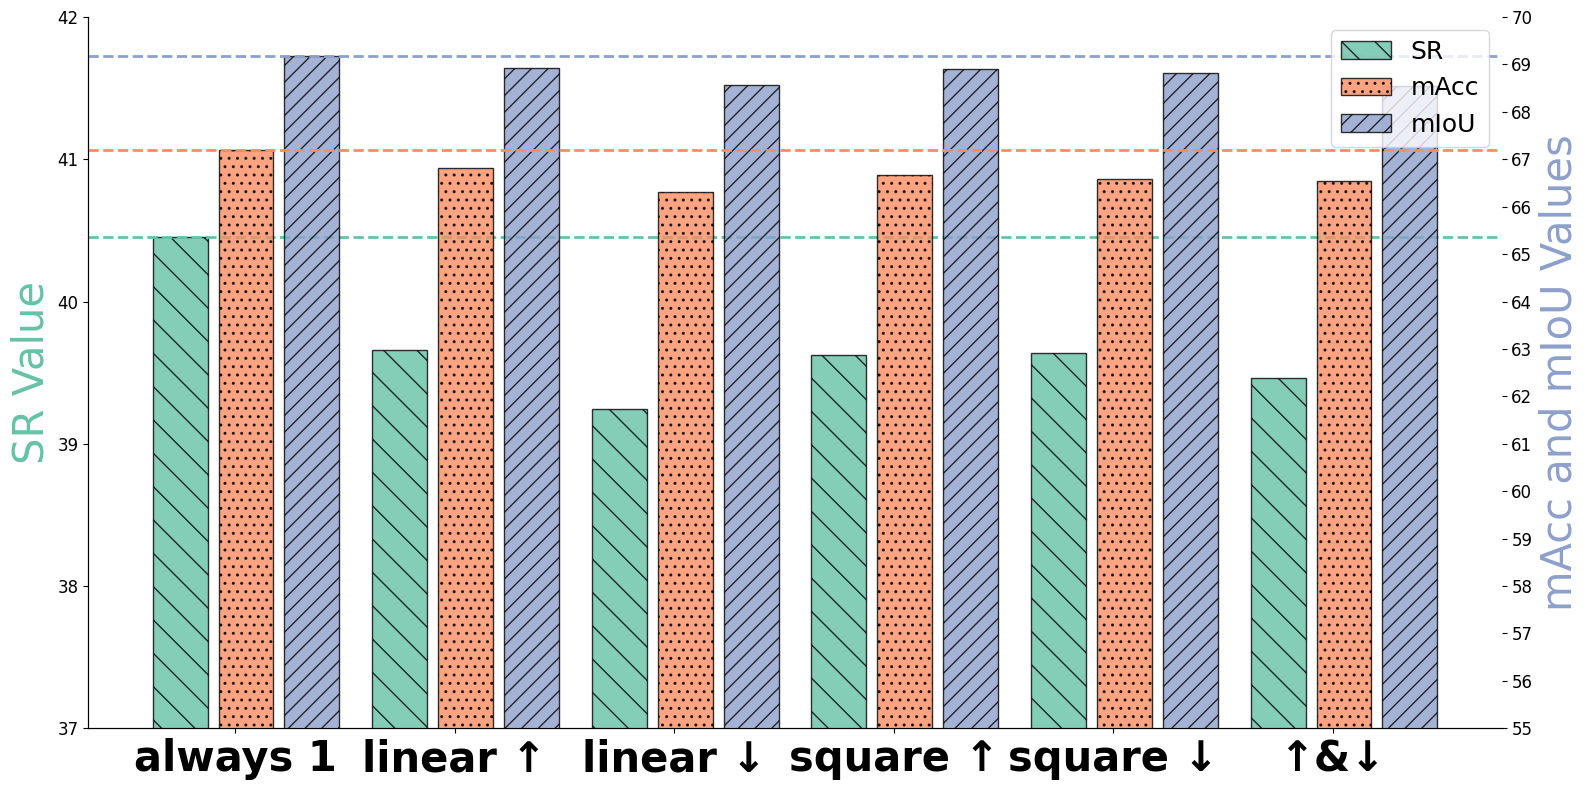
\includegraphics[width=0.45\textwidth]{figures/intx2.png}\label{fig:inxx2}}
    \caption{Ablation studies for interpolation strategy. Note: ``always 1'' indicates that $\tau$ is initialized to `1'; ``linear $\uparrow$'' denotes that the values in the matrix $\tau$ increase linearly, with the first column initialized to `1' and the last column set to `6' in \Cref{fig:inxx1}, with a gradual linear increase in between, and from `0' to `1' in \Cref{fig:inxx2}; ``linear $\downarrow$'' represents the reverse process. ``square $\uparrow$'' indicates that the value of $\tau$ increases following a square progression. ``$\uparrow$ \& $\downarrow$'' refers to a variation similar to our gradient loss weights, where the value first increases linearly and then decreases. }
    \label{fig:inxx3}
\end{figure}

\begin{table}[t]
\centering
\caption{Ablation study on the role of classifier type on COIN dataset.}
\vspace{-3mm}
\scalebox{0.92}{
\begin{tabular}{lccccccc}
\toprule
& \multicolumn{3}{c}{$T$ = 3} & & \multicolumn{3}{c}{$T$ = 4} \\ 
\cline{2-4} \cline{6-8}
{Models}          & SR$\uparrow$ & mAcc$\uparrow$   & mIoU$\uparrow$  &   & SR$\uparrow$    & mAcc$\uparrow$   & mIoU$\uparrow$  \\ \midrule
{PDPP (Res-MLP)}             &   21.33   &   45.62 & 51.82 & & 14.41 & 44.10 & 51.39 \\
{PDPP (Transformer)} & \underline{24.02} & \underline{48.03} & \underline{55.21} & & \underline{17.36} & \underline{46.12} & \underline{55.82} \\
{MTID (Transformer)} &  \bf 28.84 & \bf 50.44 & \bf 57.86 & & \bf 21.64 & \bf 48.06 & \bf 59.52 \\
\bottomrule
\end{tabular}
}
\label{tab:classifier_coin}
\end{table}




\textbf{More Interpolation Strategies.} We experimented with both linear and non-linear strategies, as shown in \Cref{fig:inxx3}. In \Cref{fig:inxx1}, we found that using a maximum value of `6' led to poor results, particularly for the ``square $\uparrow$'' and ``square $\downarrow$'' strategies, indicating a significant deviation from the desired final value. When we reduced the maximum value to `1', the results still remained unsatisfactory, suggesting that the final value of $\tau$ consistently converged around `1', resulting in sub-optimal performance.



\begin{figure}[ht]
    \centering
    \subfloat[Ablation studies on the number of transformer encoder block layers.]{
        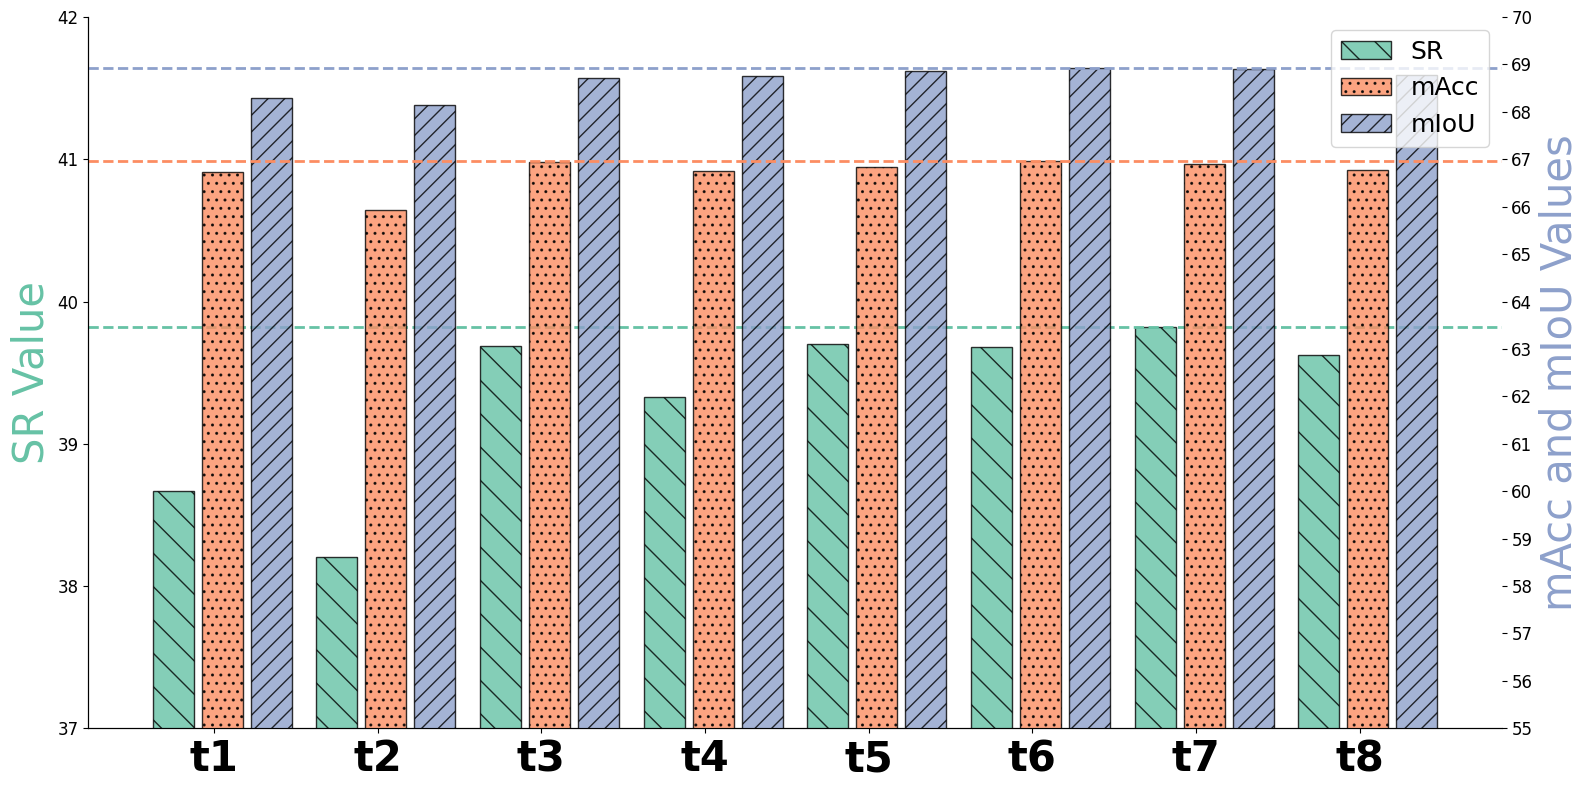
\includegraphics[width=0.48\textwidth, keepaspectratio]{figures/ab1.png}
        \label{fig:num_trans}
    }
    \hfill
    \subfloat[Ablation studies on the scale of mask loss.]{
        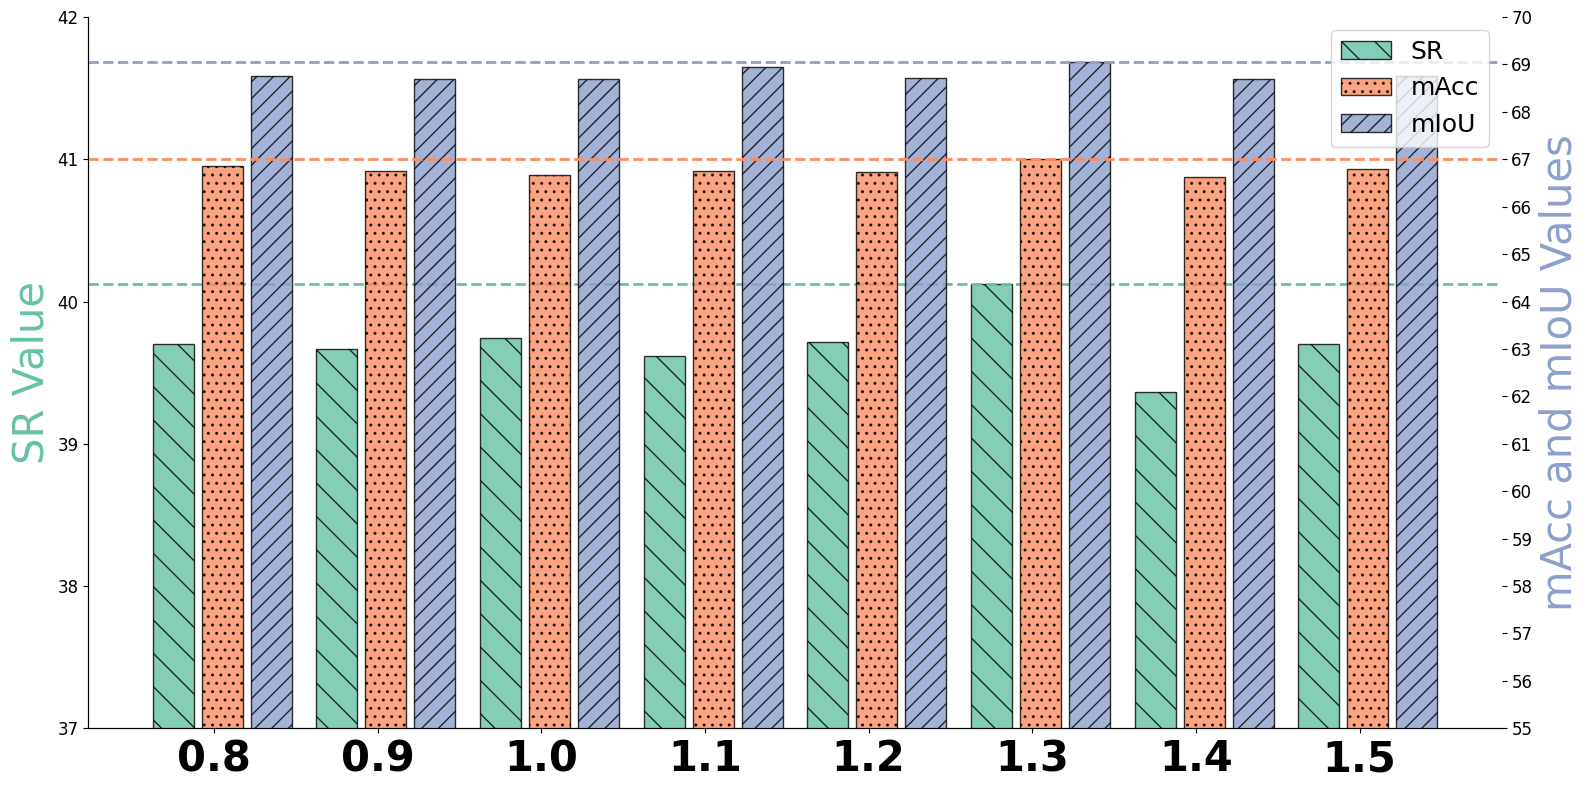
\includegraphics[width=0.48\textwidth, keepaspectratio]{figures/ab2.png}
        \label{fig:scale_mask}
    }
    \hfill
    \subfloat[Ablation studies on the weights coefficient of loss.]{
        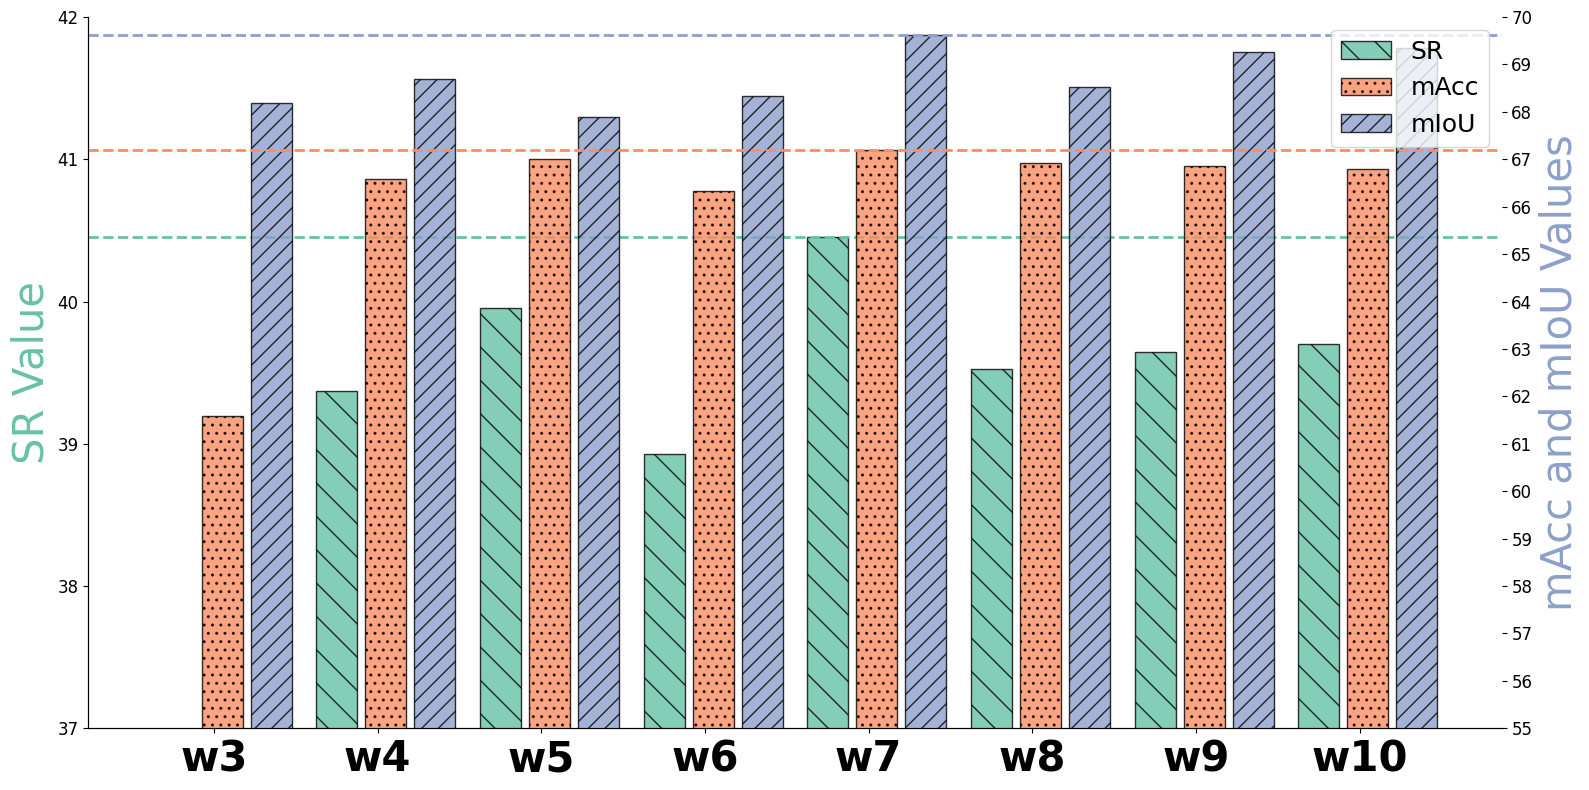
\includegraphics[width=0.48\textwidth, keepaspectratio]{figures/ab3.png}
        \label{fig:wei_coef}
    }
    \caption{Combined ablation studies of different coefficients. Note: ``t1'' refers to the number of transformer encoder layers in \Cref{fig:num_trans}; ``0.8'' represents the value of $\rho$ in loss function in \Cref{fig:scale_mask}; and ``w3'' indicates the value of the gradient-weighted loss $w_0$ in \Cref{fig:wei_coef}.   }
    \label{fig:combined}
\end{figure}


\begin{table}[htbp]
\centering
\caption{Comparisons of mIoU on COIN and NIV datasets.}
\scalebox{0.88}{
\begin{tabular}{>{\arraybackslash}p{2cm} cc cc >{\arraybackslash}p{2cm} cc cc}
\toprule
& \multicolumn{2}{c}{$T$ = 3} & \multicolumn{2}{c}{$T$ = 4} &
& \multicolumn{2}{c}{$T$ = 3} & \multicolumn{2}{c}{$T$ = 4} \\ 
\cline{2-5} \cline{7-10}
{Models(COIN)}  & \multicolumn{2}{c}{mIoU$\uparrow$} & \multicolumn{2}{c}{mIoU$\uparrow$} &
{Models(NIV)}   & \multicolumn{2}{c}{mIoU$\uparrow$} & \multicolumn{2}{c}{mIoU$\uparrow$} \\ 
\midrule
Random       & \multicolumn{2}{c}{\color{gray}2.47}    & \multicolumn{2}{c}{\color{gray}2.32}    &
Random       & \multicolumn{2}{c}{\color{gray}6.09}    & \multicolumn{2}{c}{\color{gray}5.84}    \\
DDN          & \multicolumn{2}{c}{\color{gray}64.78}   & \multicolumn{2}{c}{\color{gray}68.06}   &
DDN          & \multicolumn{2}{c}{\color{gray}56.56}   & \multicolumn{2}{c}{\color{gray}53.84}   \\
P$^3$IV      & \multicolumn{2}{c}{\color{gray}76.31}   & \multicolumn{2}{c}{\color{gray}70.53}   &
Ext-GAIL     & \multicolumn{2}{c}{\color{gray}65.93}   & \multicolumn{2}{c}{\color{gray}53.84}   \\
EGPP         & \multicolumn{2}{c}{\bf \color{gray}84.95} & \multicolumn{2}{c}{\bf \color{gray}84.72} &
P$^3$IV      & \multicolumn{2}{c}{\color{gray}74.29}   & \multicolumn{2}{c}{\color{gray}67.29}   \\
PDPP         & \multicolumn{2}{c}{\underline{51.82}}   & \multicolumn{2}{c}{51.39}               &
EGPP         & \multicolumn{2}{c}{\color{gray}75.81}   & \multicolumn{2}{c}{\color{gray}74.90}   \\
KEPP         & \multicolumn{2}{c}{51.72}               & \multicolumn{2}{c}{\underline{53.27}}   &
KEPP         & \multicolumn{2}{c}{\bf \color{gray}86.67} & \multicolumn{2}{c}{\bf \color{gray}91.49} \\
SCHEMA       & \multicolumn{2}{c}{\color{gray}\underline{83.83}} & \multicolumn{2}{c}{\color{gray}\underline{83.47}} &
SCHEMA       & \multicolumn{2}{c}{\color{gray}\underline{76.77}} & \multicolumn{2}{c}{\color{gray}\underline{76.75}} \\
\midrule
MTID (Ours)  & \multicolumn{2}{c}{\bf 59.58}           & \multicolumn{2}{c}{\bf 60.78}           &
MTID (Ours)  & \multicolumn{2}{c}{\bf 56.49}           & \multicolumn{2}{c}{\bf 58.50}           \\
\bottomrule
\end{tabular}
}
\label{tab:combined_miou}
\end{table}

\textbf{Results of mIoU on COIN and NIV.} \Cref{tab:combined_miou} shows that our model achieves notable improvements in mIoU on both the COIN and NIV datasets.

\textbf{Number of Transformer Encoder Layers.} \Cref{fig:num_trans} shows the scores of three metrics across different numbers of layers in the transformer encoder blocks. The results indicate that using fewer layers (1 or 2) results in a significant drop in performance, with SR being the most adversely affected. As the number of layers increases, the metrics stabilize, with notable improvements, especially in SR, which shows a significant positive shift at 6 and 7 layers. In contrast, mAcc and mIoU show more subtle variations, with slight positive changes as the number of layers increases, reflecting a steady trend. These results suggest that an optimal configuration of 6 or 7 layers delivers the best overall performance.

\textbf{Scale of Mask Loss.} \Cref{fig:scale_mask} illustrates the impact of different values of $\rho$ on the loss function. We observe that when $\rho=1.3$, the scores are higher than for other values. Therefore, we adopt this value.

\textbf{Weight Coefficient of Loss.} \Cref{fig:wei_coef} shows the results for different values of $w_0$, the weight coefficient of the loss function. The results indicate that when $w_0$ is set to 7, the scores are higher than for other values.


\section{Further Discussions}
This section offers further discussion on related works and presents insights that were excluded from the main paper due to space limitations. 

\textbf{Limitations.} The limitations of our method are as follows. First, while the logical consistency between the actions generated by our model is generally strong, there is no guarantee of perfect alignment with the task. Mismatches were observed during the experiments, which is a common issue in procedure planning models. This challenge arises because the labels for multi-task and multi-action tasks in the dataset are replaced by data IDs, which may lead to issues with numerical calculations. 
Second, we found that our model cannot entirely eliminate repeated action predictions, which is a limitation in its current design.

\textbf{Comparison Across Supervision Strategies and Mid-State Handling.} Our MTID model introduces several innovations that set it apart in terms of how it handles supervision and mid-state action prediction:
(1) \textit{Supervision Approach: Weak vs. Full Supervision}:
% \textit{Compared to DDN}~\citep{chang2020procedure}, \textit{PlaTe}~\citep{sun2022plate}, and \textit{Ext-GAIL}~\citep{bi2021procedure}: 
DDN, PlaTe, and Ext-GAIL rely on fully supervised learning, requiring extensive annotations to model temporal dynamics. In contrast, MTID uses a weakly supervised approach with a latent space temporal interpolation module, capturing mid-state information without detailed annotations. Its diffusion process and latent interpolation offer finer-grained supervision for intermediate steps, outperforming Ext-GAIL and DDN in long-term predictions.
(2) \textit{Intermediate State Supervision and Logical Structure}:
% \textit{Compared to PDPP}~\citep{wang2023pdpp} and \textit{Skip-Plan}~\citep{li2023skip}: 
PDPP uses task labels to bypass intermediate state supervision, and Skip-Plan reduces uncertainty by skipping uncertain intermediate actions. However, both methods struggle to fully capture the logical structure of intermediate steps. MTID addresses this by explicitly supervising mid-state actions through latent space interpolation, ensuring that the generated sequences are both temporally logical and well-aligned with the task requirements.
(3) \textit{Handling of External Knowledge and Probabilistic Guidance}:
% \textit{Compared to P3IV}~\citep{zhao2022p3iv} and \textit{KEPP}~\citep{nagasinghe2024not}: 
P3IV leverages natural language instructions for weak supervision, while KEPP uses a probabilistic procedural knowledge graph (P2KG) to guide the planning process. While both methods aim to improve action prediction through external guidance, MTID distinguishes itself by focusing on direct mid-state supervision via intermediate latent features from a diffusion model. This approach provides more precise control over action generation, ensuring logical consistency across the entire sequence.
(4) \textit{State Representation and Visual Alignment}:
% \textit{Compared to SCHEMA}~\citep{niu2024schema}: 
SCHEMA relies on large language models (LLMs) to describe and align state changes with visual observations, focusing on high-level state transitions. MTID, in contrast, directly uses mid-state supervision through latent space temporal interpolation, which improves visual-level supervision and enhances temporal reasoning, resulting in more accurate action sequence predictions.


\textbf{Generalization Capabilities.} Our MTID model demonstrates strong generalization across variations in action steps, object states, and environmental conditions. For action step variations, the model was evaluated with sequences of different lengths, ranging from 3 to 6 steps. The results consistently showed that MTID outperforms state-of-the-art models, leveraging its latent space temporal interpolation to capture temporal logical relationships across various step lengths. In terms of object states and environmental contexts, the benchmark datasets used for evaluation cover a wide range of topics, such as cooking, housework, and car maintenance, featuring diverse objects like fruits, drinks, and household items. For instance, the CrossTask dataset includes 133 step types across 18 tasks, while the COIN dataset features 778 step types over 180 tasks. These tests highlight MTID's ability to generalize effectively, capturing the nuances of varying object states and environmental conditions, due to its robust interpolation and diffusion framework.



\begin{figure}[htbp]
    \centering
    \subfloat[Horizon $T = 3$]{
        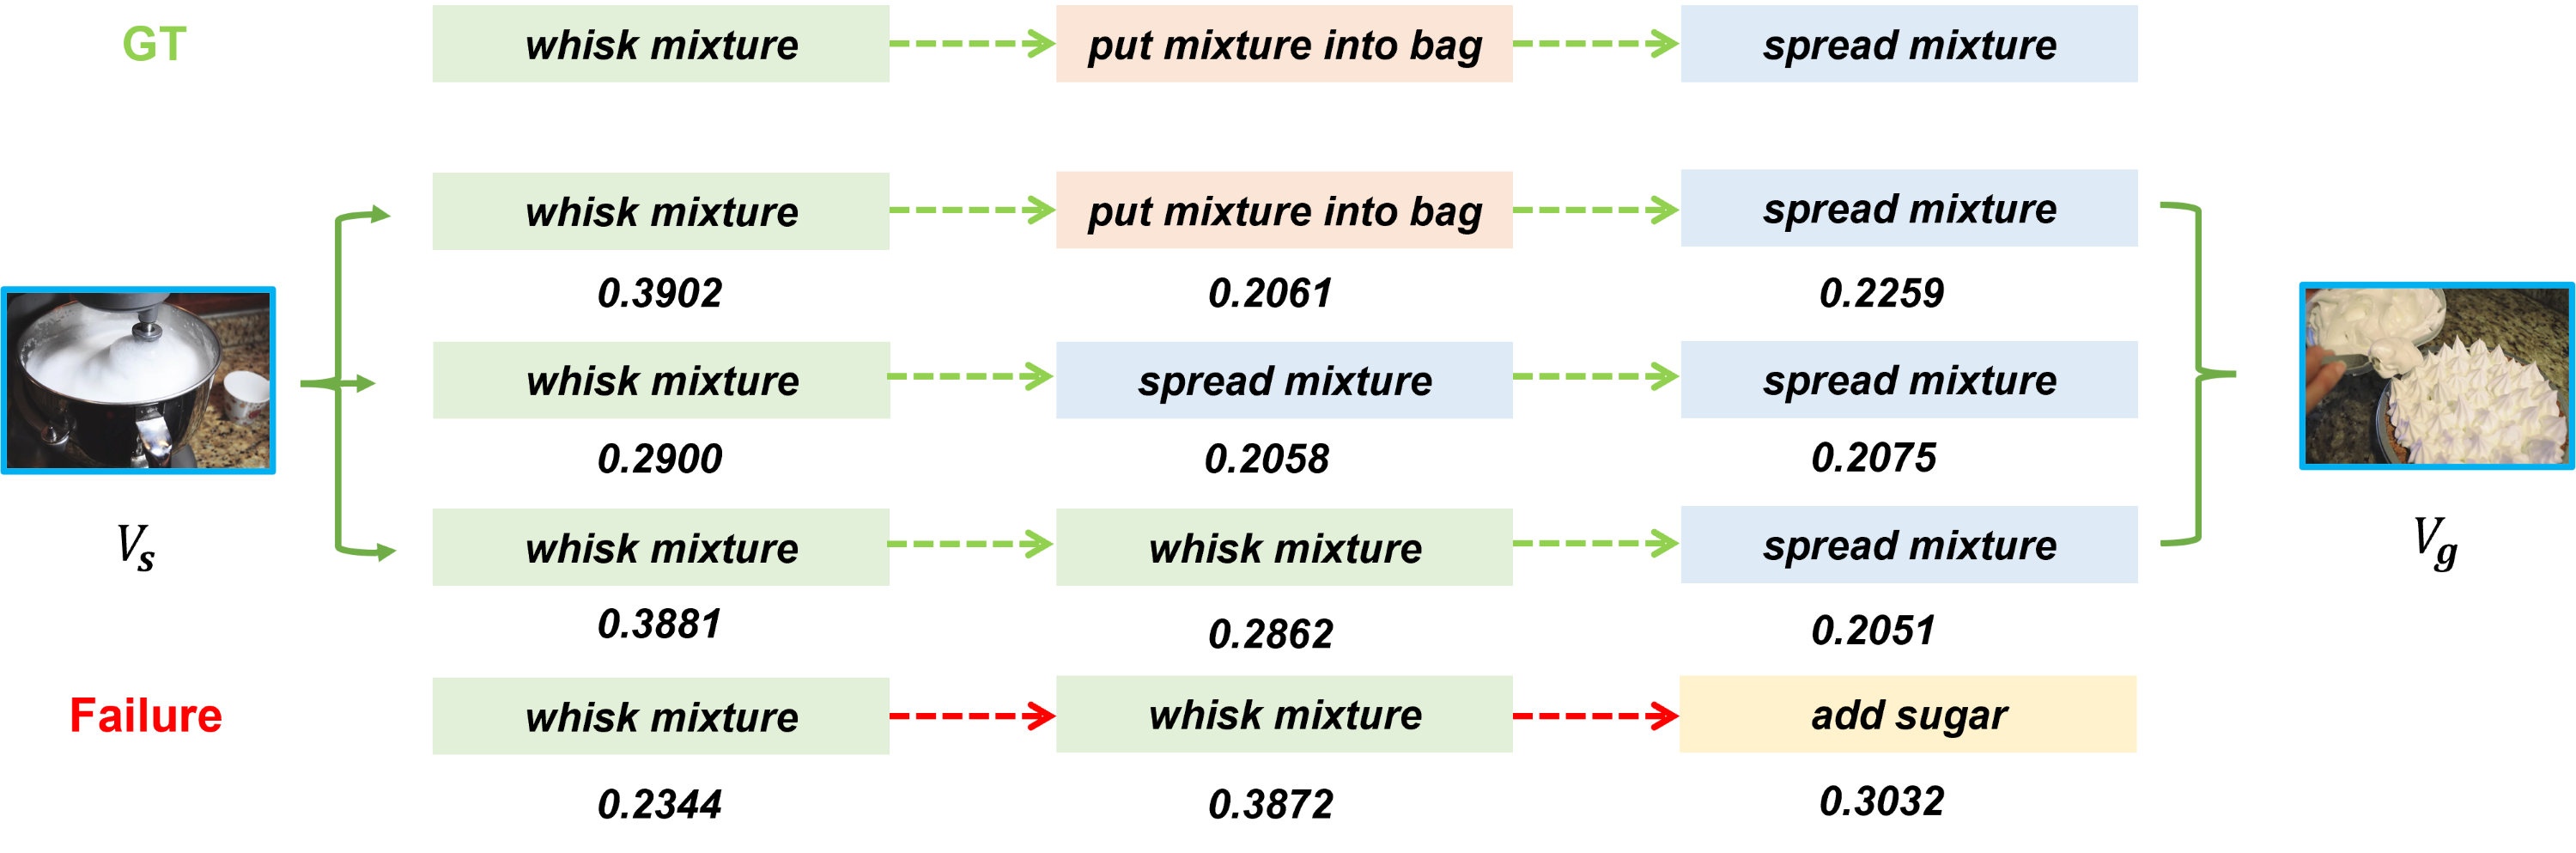
\includegraphics[width=0.95\textwidth]{figures/visualization_3.png}
        \label{fig:visual-3}
    }
    
    \vspace{1em}
    
    \subfloat[Horizon $T = 4$]{
        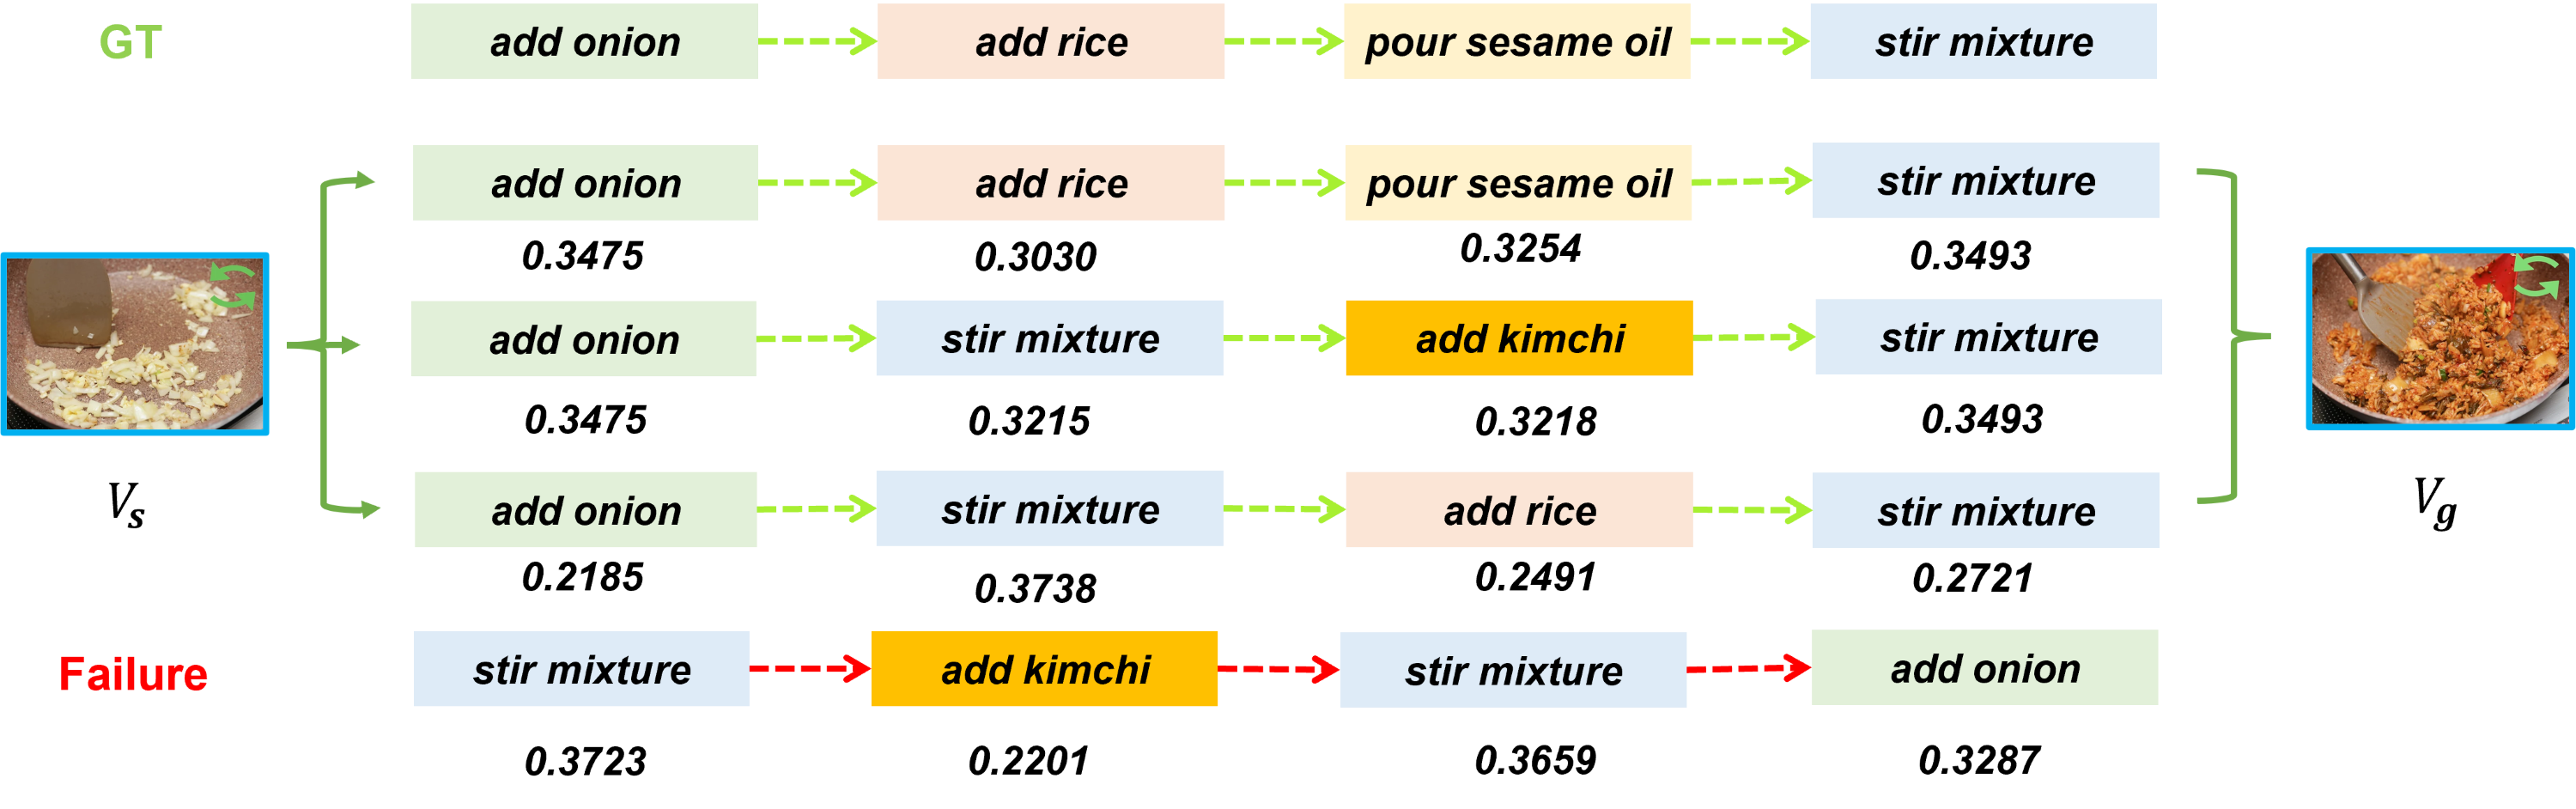
\includegraphics[width=0.95\textwidth]{figures/visualization_4.png}
        \label{fig:visual-4}
    }
    
    \vspace{1em}
    
    \subfloat[Horizon $T = 5$]{
        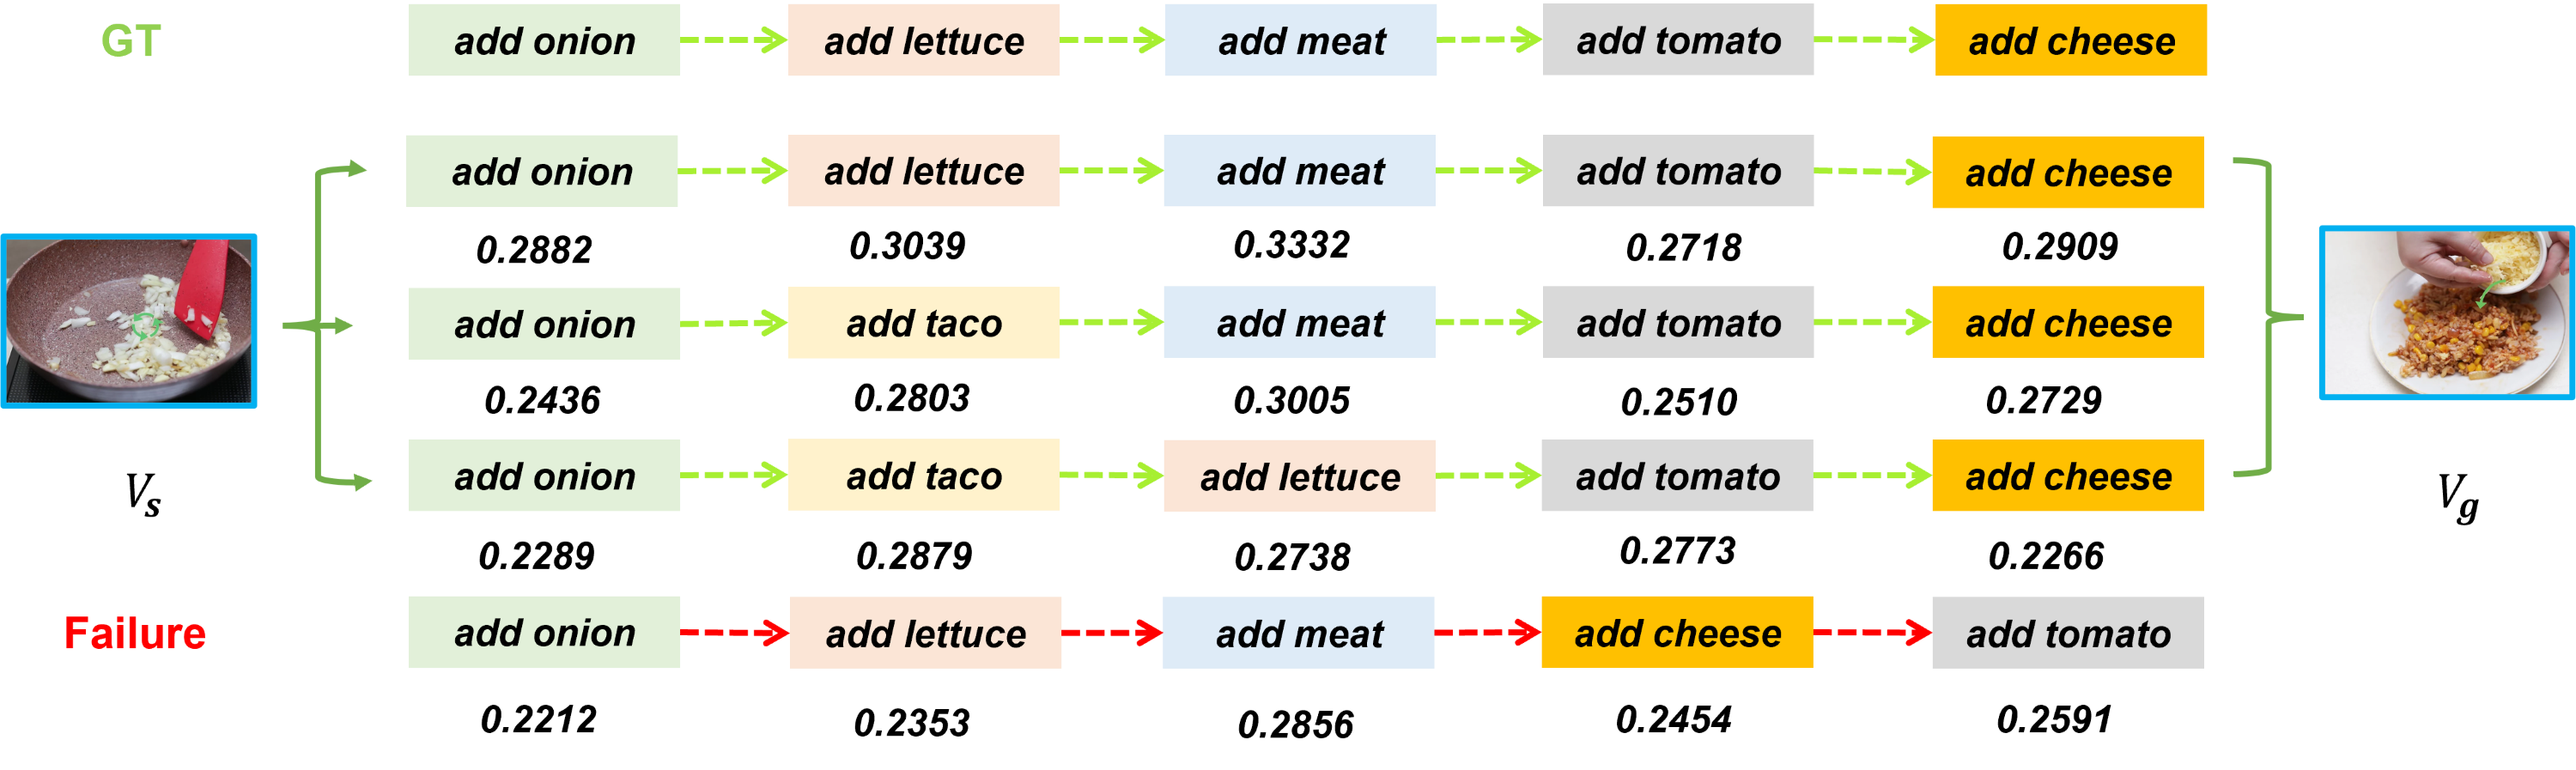
\includegraphics[width=0.95\textwidth]{figures/visualization_5.png}
        \label{fig:visual-5}
    }
    
    \vspace{1em}
    
    \subfloat[Horizon $T = 6$]{
        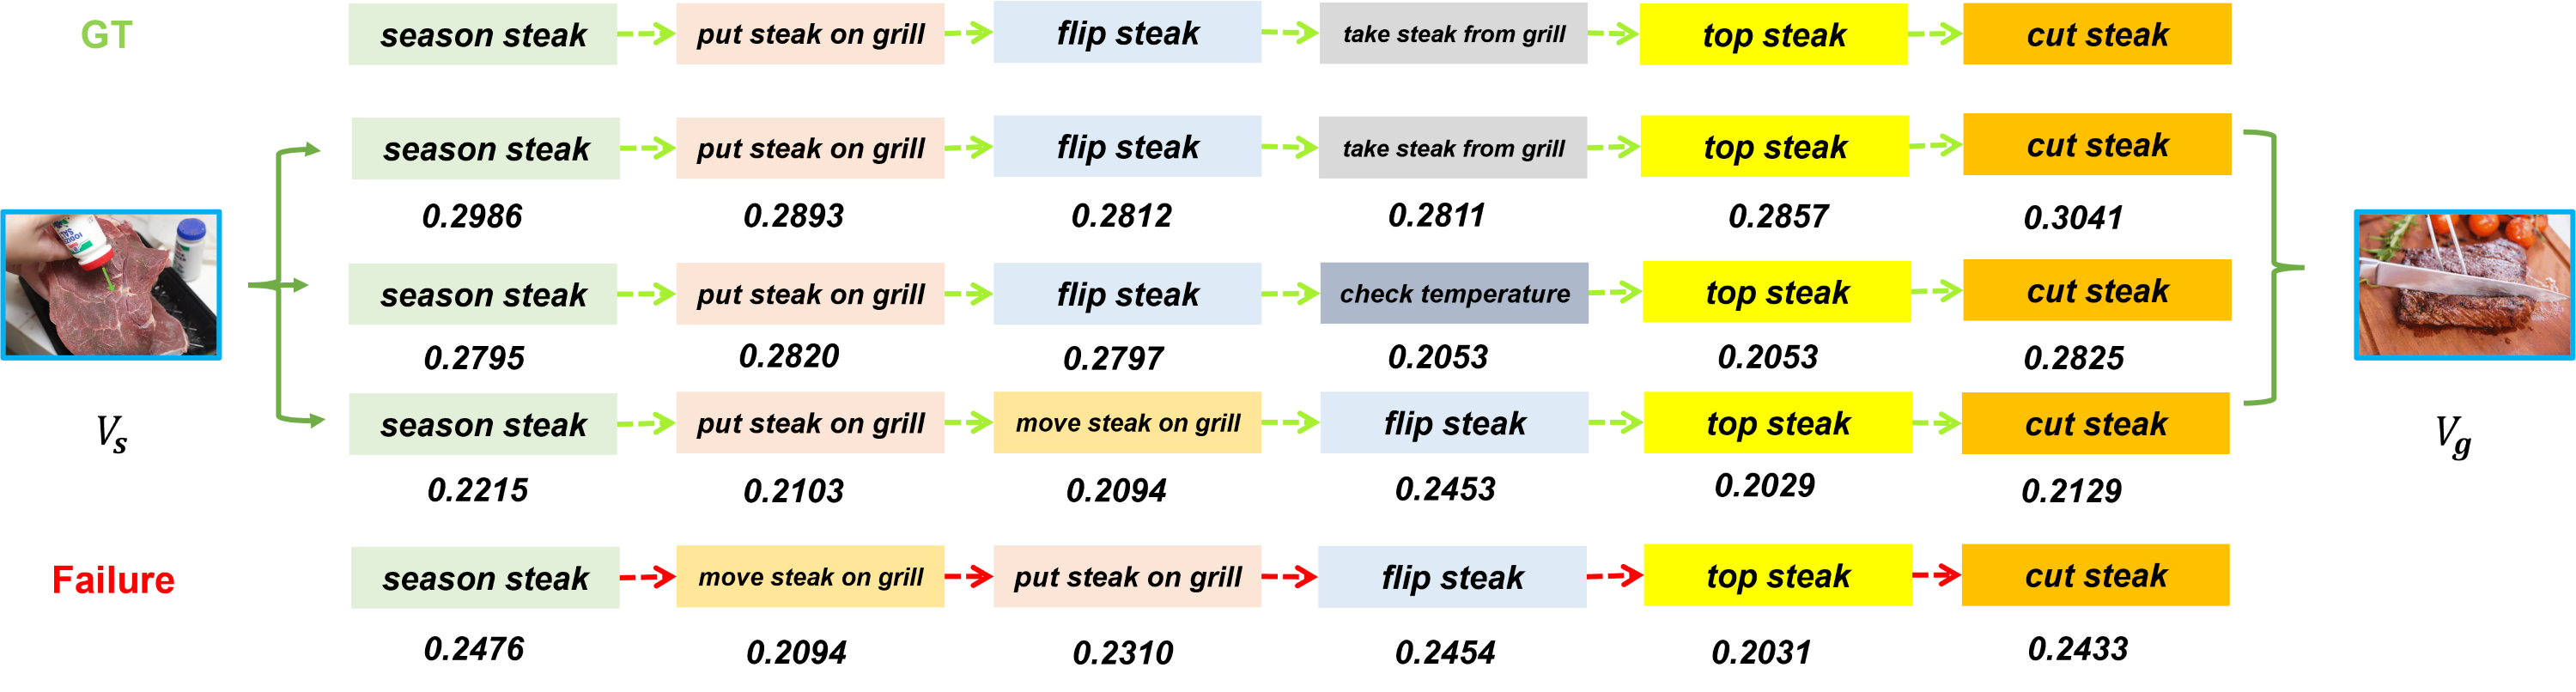
\includegraphics[width=0.95\textwidth]{figures/visualization_6.png}
        \label{fig:visual-6}
    }
    
    \caption{Visualization of diverse plans produced by our model with different horizons. Note: each figure includes images depicting the start and goal observations, the first row labeled ``GT'' showing the ground truth actions, the last row labeled ``Failure'' illustrating a plan that does not achieve the goal, and the middle rows displaying multiple reasonable plans produced by our model. These decimals represent the probability values obtained from action prediction. }
    \label{fig:visual-all}
\end{figure}